% Owner: B -- measured M2c-1 through M2c-4 only.
\paragraph{Preferential attachment (H4a).}
The conditional kernel $(k+1)^\alpha$ gives $\alpha=0.714$, with a descriptive
95\% year-bootstrap interval $[0.693,0.730]$. Twenty P3a samples yield
$0.0006\pm0.0051$ and age-only P3b yields $-0.6512\pm0.0053$.
The observed exponent exceeds all null values (empirical one-sided probability
$1/21$ per comparison, with coarse resolution). The exponent stays positive
under time splits, offsets 0.5/2 and a core venue-family subset.
\textbf{Verdict:} sublinear degree preference is supported within this corpus,
beyond the age-only reference; this does not identify a causal PA mechanism.

\paragraph{Ageing (H4b).}
Lognormal target preference is preferred to exponential, power-law and uniform
kernels, with respective $\Delta$AIC 537.8, 9,360.5 and 41,796.7.
The lognormal parameters are $(\mu,\sigma)=(1.858,1.108)$; its underlying scale
$e^\mu$ is 6.41 years. Mean age over all retained citations is 5.711 years, versus
$11.457\pm0.034$ for P3a and $5.717\pm0.018$ for calibrated P3b.
Lognormal is preferred in all three target cohorts, although recent-cohort tails
remain censored. \textbf{Verdict:} age-independent choice is inadequate;
P3b's agreement is calibration, not independent confirmation of ageing.

\begin{figure*}[t]
\centering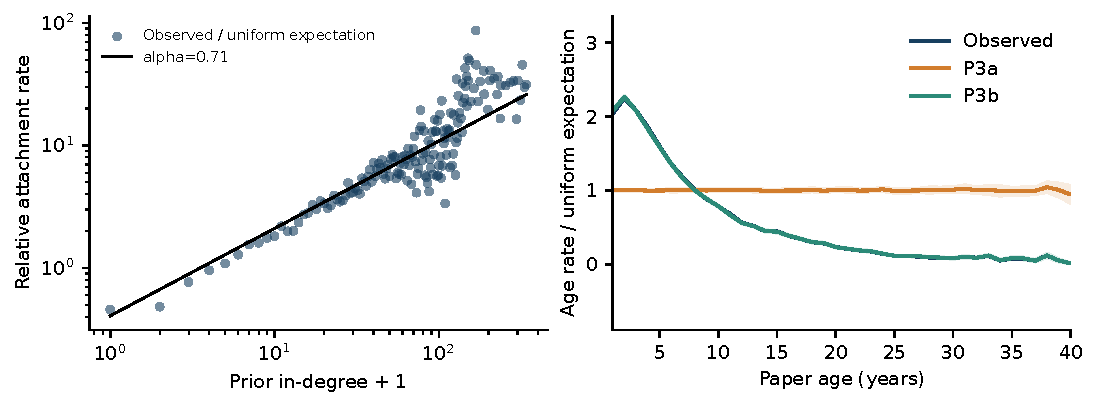
\includegraphics[width=.95\textwidth]{b_attachment_ageing.pdf}
\caption{Measured CIT attachment and exposure-adjusted age preference.
Points with at least five hits are displayed; the exponent uses all supported
classes with yearly normalization. Null bands show mean $\pm$ SD.}
\label{fig:growth}
\end{figure*}

\paragraph{Densification and diameter (H4c).}
For 1990--2020, $a=1.343$ ($R^2=0.991$), with descriptive year-resampling
interval $[1.288,1.406]$. Growth is weaker in 2005--2020 ($a=1.065$) than
1990--2004 (1.455); cutoff 2015 gives 1.427, inclusion of year ties 1.324,
and the core venue subset 1.410. Densification is superlinear edge growth,
not increasing directed density. The sampled weak-LCC effective diameter is
6 hops in every year; 64/256-source endpoint checks agree.
P3 fixes $N(t)$ and $E(t)$, hence also $a$.
\textbf{Verdict:} densification is observed, but diameter shrinkage is not
detected at the sampled 90th-percentile resolution.

\begin{figure*}[t]
\centering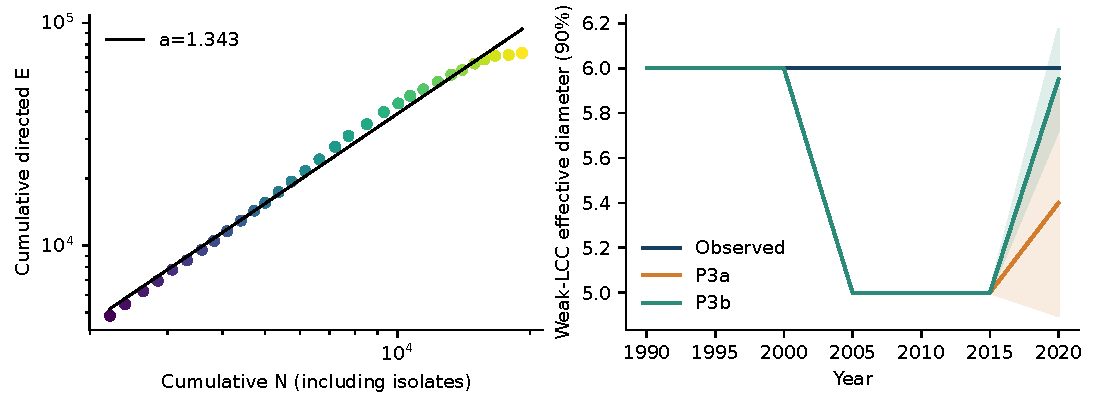
\includegraphics[width=.95\textwidth]{b_densification_diameter.pdf}
\caption{CIT cumulative growth and effective diameter. Null diameter means and
SD are estimated every five years. P3 cannot test densification significance
because its source reference counts are fixed.}
\label{fig:b-densification}
\end{figure*}

\paragraph{Citation dynamics and prediction (H4d).}
For 500 full-history fits, median WSB parameters are
$(\lambda,\mu,\sigma)=(2.717,0.834,1.238)$, median RMSLE is 0.074 and
scaled-collapse RMSE is 0.022. These are fitted-sample diagnostics.
On 500 papers selected using only their first five years, age-15 MAE is
15.144 for WSB, 17.064 for linear extrapolation and 27,588 for no-ageing PA;
at the observed 2020 endpoint it is 28.016, 27.271 and $2.79\times10^6$.
The paired MAE differences WSB minus linear have 95\% intervals
$[-4.471,0.806]$ and $[-4.764,8.128]$, both including zero. Forecast fits hit
parameter bounds for 38.6\% of papers; all remain in primary scoring.
\textbf{Verdict:} compact descriptive fits are supported, but a clear predictive
advantage over the simple linear baseline is not established. Observed-endpoint
citations are censored within-corpus counts, not lifetime impact.

\begin{figure*}[t]
\centering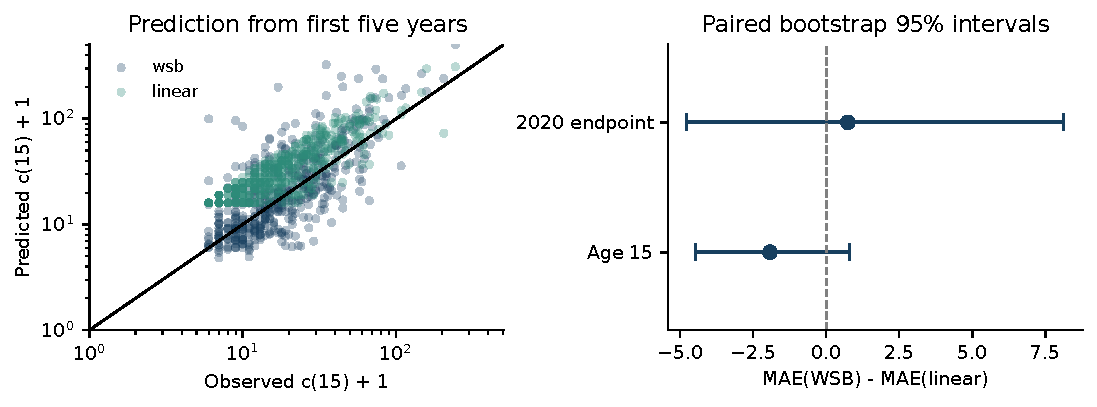
\includegraphics[width=.95\textwidth]{b_wsb_validation.pdf}
\caption{WSB held-out prediction and paired MAE differences versus linear.
Both bootstrap intervals cross zero; fitted collapse alone does not establish
long-term predictability.}
\label{fig:b-wsb-validation}
\end{figure*}
